\subsection{Dice}

Dice klassen opretter vores terninger til spillet. Altså to die-objekter. 

\begin{figure}[H]
    \centering
    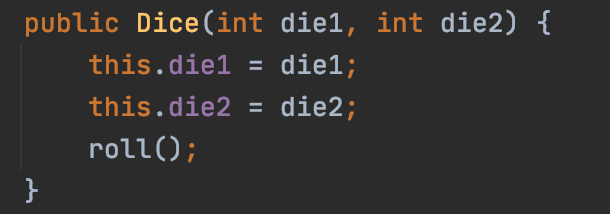
\includegraphics[width=\textwidth]{sources/7_implementering/Dice die.png}
    \caption{Die Objekter}
    \label{fig:Die}
\end{figure}
Den bruges til at få resultatet af et kast med terningerne. Man kan efter et kast se de to terningers værdier samt summen af de to, efter den giver to tilfældige værdier mellem 1 og 6. 
Klassen tjekker om de to terninger har ens værdier med getEquals-metoden. Som bruges til f.eks. at komme ud af fængsel i spillet.
\begin{figure}[H]
    \centering
    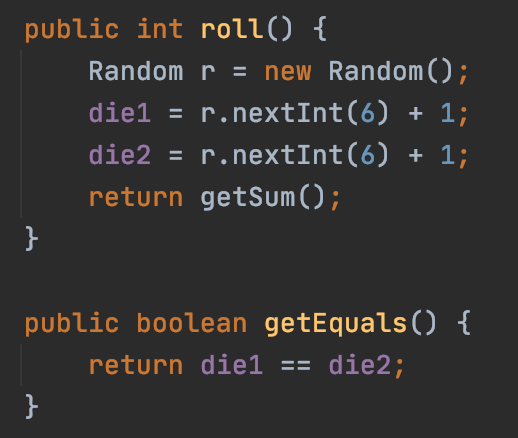
\includegraphics[width=\textwidth]{sources/7_implementering/Dice Roll_GetEquals}
    \caption{Equals og Roll metoder}
    \label{fig:diceRollEquals}
\end{figure}
Sidst har vi en række getters. En for hver terning og én til summen.
\begin{figure}[H]
    \centering
    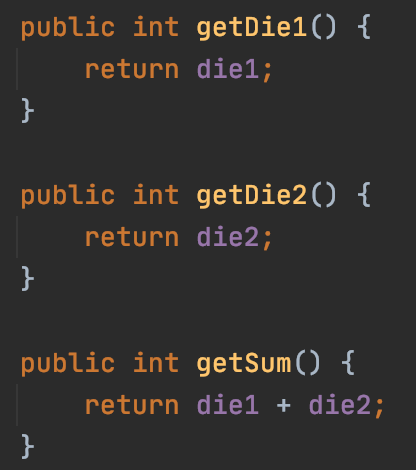
\includegraphics[width=\textwidth]{sources/7_implementering/Dice Getters.png}
    \caption{Dice Getters}
    \label{fig:DiceGetters}
\end{figure}